\documentclass[twoside,twocolumn]{article}

\usepackage{blindtext} % Package to generate dummy text throughout this template 
\usepackage{graphicx}
\usepackage[sc]{mathpazo} % Use the Palatino font
\usepackage[T1]{fontenc} % Use 8-bit encoding that has 256 glyphs
\linespread{1.05} % Line spacing - Palatino needs more space between lines
\usepackage{microtype} % Slightly tweak font spacing for aesthetics

\usepackage[english]{babel} % Language hyphenation and typographical rules

\usepackage[hmarginratio=1:1,top=32mm,columnsep=20pt]{geometry} % Document margins
\usepackage[hang, small,labelfont=bf,up,textfont=it,up]{caption} % Custom captions under/above floats in tables or figures
\usepackage{booktabs} % Horizontal rules in tables

\usepackage{lettrine} % The lettrine is the first enlarged letter at the beginning of the text

\usepackage{enumitem} % Customized lists
\setlist[itemize]{noitemsep} % Make itemize lists more compact

\usepackage{abstract} % Allows abstract customization
\renewcommand{\abstractnamefont}{\normalfont\bfseries} % Set the "Abstract" text to bold
\renewcommand{\abstracttextfont}{\normalfont\small\itshape} % Set the abstract itself to small italic text

\usepackage{titlesec} % Allows customization of titles
\renewcommand\thesection{\Roman{section}} % Roman numerals for the sections
\renewcommand\thesubsection{\roman{subsection}} % roman numerals for subsections
\titleformat{\section}[block]{\large\scshape\centering}{\thesection.}{1em}{} % Change the look of the section titles
\titleformat{\subsection}[block]{\large}{\thesubsection.}{1em}{} % Change the look of the section titles

\usepackage{fancyhdr} % Headers and footers
\pagestyle{fancy} % All pages have headers and footers
\fancyhead{} % Blank out the default header
\fancyfoot{} % Blank out the default footer
\fancyhead[C]{El Aseguramiento de la Calidad de Software  $\bullet$ Mayo 2019 $\bullet$ } % Custom header text
\fancyfoot[RO,LE]{\thepage} % Custom footer text

\usepackage{titling} % Customizing the title section

\usepackage{hyperref} % For hyperlinks in the PDF

%----------------------------------------------------------------------------------------
%	TITLE SECTION
%----------------------------------------------------------------------------------------

\setlength{\droptitle}{-4\baselineskip} % Move the title up

\pretitle{\begin{center}\Huge\bfseries} % Article title formatting
\posttitle{\end{center}} % Article title closing formatting
\title{ Comparativa de Paradigmas de programación utilizando metricas de calidad} % Article title
\author{Yaneth Aquino,Bianca Chura ,Adnner Esperilla y Johanna Torres}
\date{\today} % Leave empty to omit a date
\renewcommand{\maketitlehookd}{%
\begin{abstract}
\noindent La  calidad  es  un  concepto  relativo  y  multidimensional,  referido  a  las  expectativas  y  cualidades solicitados por el cliente, a su vez, está ligada a restricciones y compromisos (presupuesto y tiempo de  desarrollo,  entre  otros).  Sin  embargo,  existe  algo  que  nadie  puede  negar,  cuando  algo  es  de calidad  suele  pasar  desapercibido,  pero,  por  el  contrario,  la  mala  calidad  es  algo  que destaca negativamente.
\end{abstract}
}
%----------------------------------------------------------------------------------------

\begin{document}

% Print the title
\maketitle

%----------------------------------------------------------------------------------------
%	ARTICLE CONTENTS
%----------------------------------------------------------------------------------------

\section{Introduccion}

\lettrine[nindent=0em,lines=3]{P}ara  producir  software  de  calidad  y  cumplir  con  la  expectativas  de  nuestros  usuarios es que existen diferentes métricas de calidad de software. Métricas de calidad de software es un conjunto de medidas utilizadas para estimar la calidad de un proyecto   a   desarrollar,   entre   otros   conceptos,   y   que   permiten   comparar   o   planificar   estas aplicaciones. son
diseñados, especificados e implementados con el propósito de estar al día con la evolución de la programación
paradigmas (por ejemplo, imperativos, orientados a objetos, orientados a aspectos, reflexivos y funcionales, por nombrar algunos).
%------------------------------------------------
%------------------------------------------------
\section{Desarrollo}

\subsection{Ruby}
Ruby es un lenguaje de programación dinámico,{\bf \underline {reflexivo y orientado a objetos}}  de propósito general que combina sintaxis
inspirado por Perl con características similares a Smalltalk. Ruby se originó en Japón a mediados de la década de 1990 y fue
desarrollado y diseñado por Yukihiro "Matz" Matsumoto. Ruby es un lenguaje de programación puro orientado a objetos
con una sintaxis súper limpia que hace que la programación sea elegante y divertida. Ruby combina con éxito Smalltalk's
elegancia conceptual, la facilidad de uso y aprendizaje de Python, y el pragmatismo de Perl. Ruby ha comenzado a convertirse en
popular en todo el mundo.Ruby soporta múltiples paradigmas de programación,incluyendo {\bf \underline {funcionales, orientados a objetos,}}
{\bf \underline {imperativos,y reflexivo.}}También cuenta con un sistema de tipo dinámico y gestión automática de la memoria.
En  Ruby,  Rubocop,  Rubicritic,  Bullet  son  algunas  que  pueden  salvarnos  el  día  y ayudarnos a optimizar nuestro código.
\begin{center}
	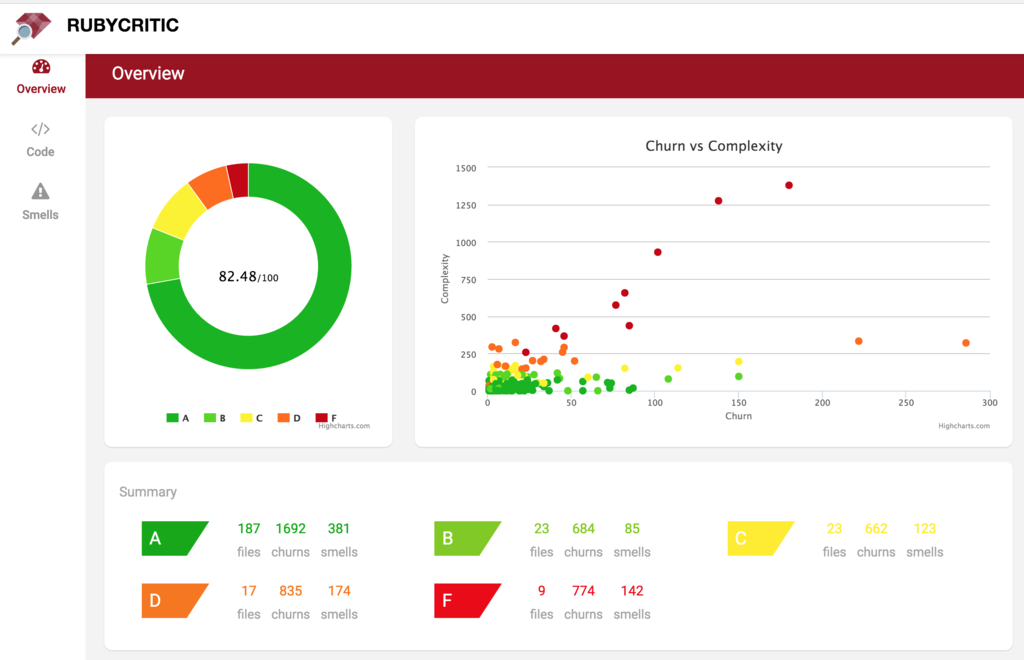
\includegraphics[width=7cm]{./Imagenes/ruby} 
	\end{center}
\subsection {RubyCritic}
\begin{itemize}
Es una herramienta para el análisis estático del código ruby ,envuelve gemas de análisis estático como Reek , Flay y Flog para proporcionar un informe de calidad de su código Ruby.
Cada una de estas gemas está internamente envuelta como un analizador , con una colección de AnalysedModule s, que nos dan cálculos de métricas clave.
\end{itemize}
\subsection {Métricas principales Ruby}
\begin{itemize}
\item la rotación
\item la complejidad
\item el costo 
\item calificación
\end{itemize}
\subsection {El resultado de RubyCritic le dará cuatro valores para ayudarlo a juzgar su código}
 
\begin{itemize}
\item  Ejemplo:para proporcionar un informe de calidad de su código Ruby
\\ \textbf{ Puntuación : un número genérico que representa la calidad general del código analizado }
\\ \ Esto es básicamente un promedio del costo calculado de cada archivo.
\\ \textbf{ Churn : número de veces que se cambió un archivo}
\\ \ Churn es muy simple de calcular: es la cantidad de veces que se confirmó el archivo.
\begin{center}
	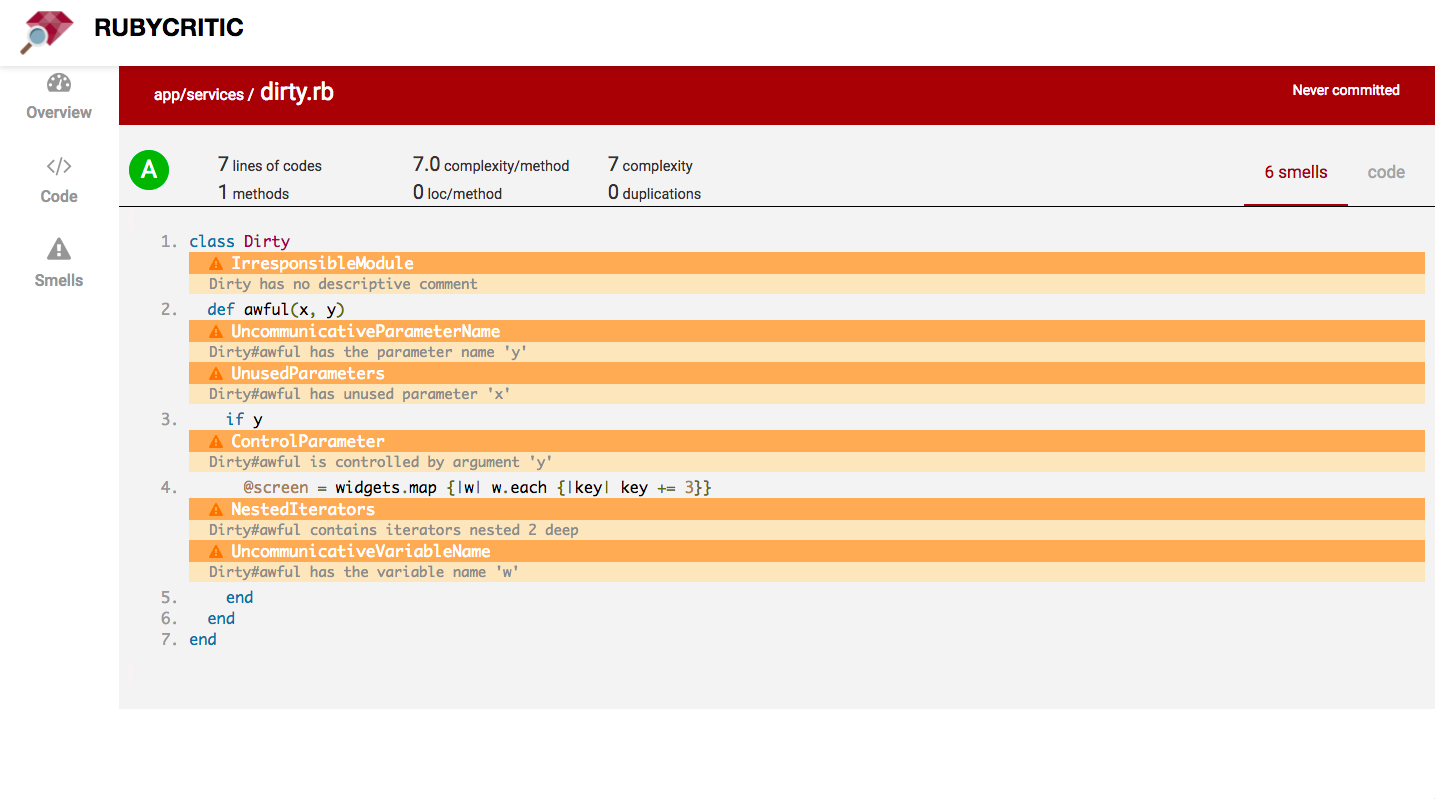
\includegraphics[width=7cm]{./Imagenes/5} 
	\end{center}
\\ \textbf{ Complejidad : cantidad de dolor en su código}
\begin{center}
	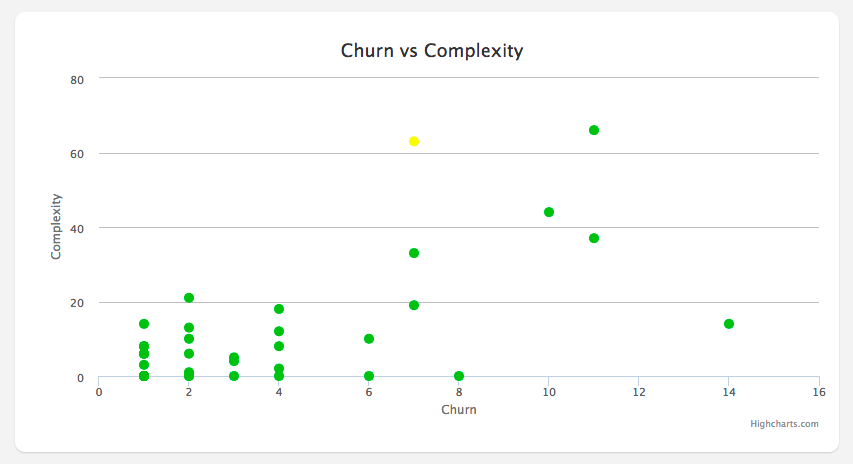
\includegraphics[width=7cm]{./Imagenes/6} 
	\end{center}
\\ \textbf{ Calificación : la calificación asignada a un archivo}
\\ \ La calificación es simplemente una conversión del costo calculado a una letra.
\begin{center}
	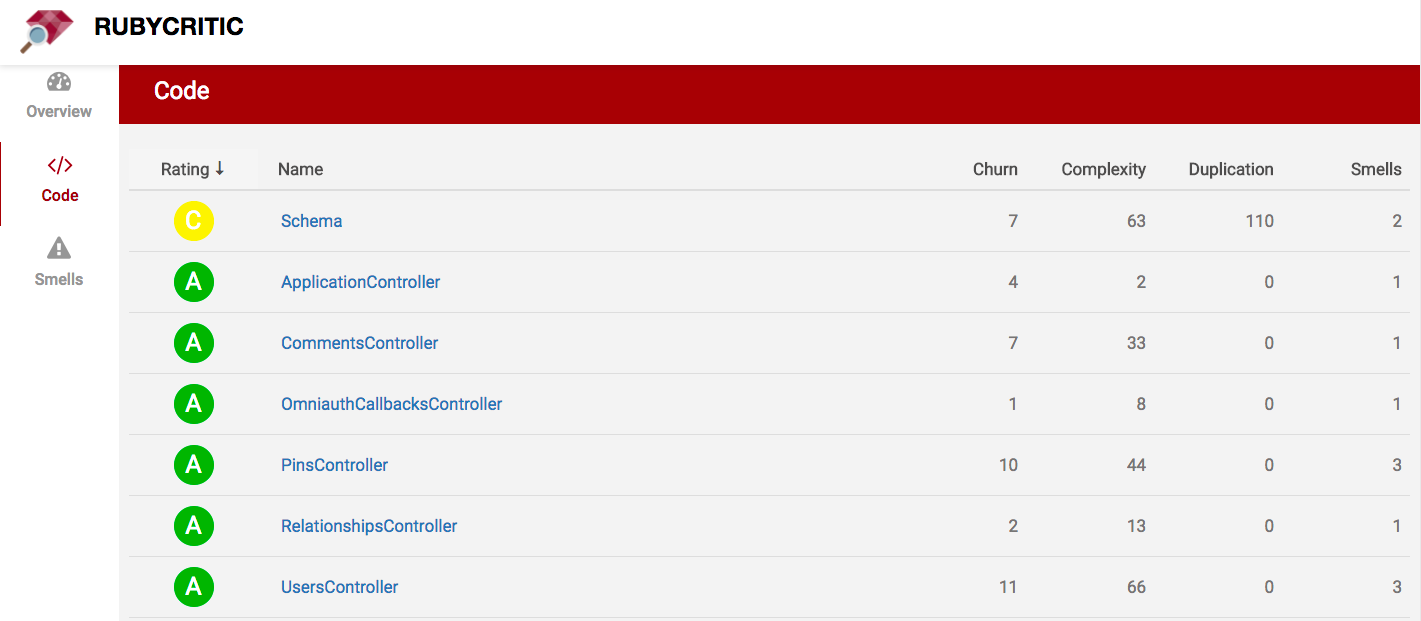
\includegraphics[width=7cm]{./Imagenes/rating} 
	\end{center}
\end{itemize}

\section{Conclusiones}
Es importante tomar decisiones tecnológicas en el momento adecuado y por las razones correctas. Buen negocio
las decisiones proporcionan a las buenas personas las herramientas de apoyo adecuadas para que puedan producir buenos productos.
Cuando se trata de desarrollo de software, lidiar con problemas de lenguaje difíciles de frente es una
requisito para el gerente visionario de hoy. Cuando se combina con otra ingeniería de software
consideraciones, una buena decisión de lenguaje puede apoyar el desarrollo de software rentable.


%---------------------------------------------------------------------------------------- 
%----------------------------------------------------------------------------------------
%	REFERENCE LIST
%----------------------------------------------------------------------------------------

\begin{thebibliography}{99} % Bibliography - this is intentionally simple in this template

 
\newblock - Al-Qahtani, S. S., Pietrzynski, P., Guzman, L. F., Arif, R., & Tevoedjre, A. (2010). Comparing selected criteria of programming languages java, php, c++, perl, haskell, aspectj, ruby, cobol, bash scripts and scheme revision 1.0-a team cplgroup comp6411-s10 term report. arXiv preprint arXiv:1008.3434.
\newblock - https://subvisual.com/blog/posts/19-solid-principles-in-ruby/
\newblock - https://github.com/whitesmith/rubycritic
\newblock - HASP. 2008. Tim Chevalier, Darin Morrison, Rebekah Leslie, Tom Harke, John Matthews, Brian Huffman, Andrew McCreight, Mark Jones, Andrew Tolmach, Peter White, James Hook. The High-Assurance Systems Programming.  http://hasp.cs.pdx.edu/overview.html (accessed July 13, 2010)
\newblock - Ruby Programming Language. About Ruby. Available at http://www.ruby-lang.org/en/about/. 
\newblock - R. Garcia, J. Jarvi, A. Lumsdaine, J. Siek, and J. Willcock. A Comparative Study of Language Support for Generic Programming. Open Systems Lab, Indiana University Bloomington, IA. November 2003
\newblock 
\end{thebibliography}

%----------------------------------------------------------------------------------------

\end{document}
